\documentclass[11pt,fleqn]{book}
\usepackage[letterpaper]{geometry}
\usepackage{graphicx}    % needed for including graphics e.g. EPS, PS
\usepackage{amsmath}
\usepackage{xfrac}
\usepackage{listings}
\usepackage{hyperref}
\usepackage{wrapfig}
\usepackage{empheq}

%\usepackage[print]{booklet}

% To use UTF-8 characters
\usepackage[utf8x]{inputenc}
% \DeclareUnicodeCharacter{207A}{$^+$}
% \DeclareUnicodeCharacter{207B}{$^-$}



% color def PYTHON CODE
\usepackage{color}
\definecolor{darkred}{rgb}{0.6,0.0,0.0}
\definecolor{darkgreen}{rgb}{0,0.50,0}
\definecolor{lightblue}{rgb}{0.0,0.42,0.91}
\definecolor{orange}{rgb}{0.99,0.48,0.13}
\definecolor{grass}{rgb}{0.18,0.80,0.18}
\definecolor{pink}{rgb}{0.97,0.15,0.45}

% listings
\usepackage{listings}

\renewcommand{\lstlistingname}{\textbf{Code}}% Listing -> Algorithm
\renewcommand{\lstlistlistingname}{List of \lstlistingname s}% List of Listings -> List of Algorithms

% General Setting of listings
\lstset{
	aboveskip=1em,
	breaklines=true,
	abovecaptionskip=-6pt,
	captionpos=t,
	escapeinside={\%*}{*)},
	frame=single,
	numbers=left,
	numbersep=15pt,
	numberstyle=\small,
}
% 0. Basic Color Theme
\lstdefinestyle{colored}{ %
	basicstyle=\ttfamily,
	backgroundcolor=\color{white},
	commentstyle=\color{green}\itshape,
	keywordstyle=\color{blue}\bfseries\itshape,
	stringstyle=\color{red},
}
% 1. General Python Keywords List
\lstdefinelanguage{PythonPlus}[]{Python}{
	morekeywords=[1]{,as,assert,nonlocal,with,yield,self,True,False,None,} % Python builtin
	morekeywords=[2]{,__init__,__add__,__mul__,__div__,__sub__,__call__,__getitem__,__setitem__,__eq__,__ne__,__nonzero__,__rmul__,__radd__,__repr__,__str__,__get__,__truediv__,__pow__,__name__,__future__,__all__,}, % magic methods
	morekeywords=[3]{,object,type,isinstance,copy,deepcopy,zip,enumerate,reversed,list,set,len,dict,tuple,range,xrange,append,execfile,real,imag,reduce,str,repr,}, % common functions
	morekeywords=[4]{,Exception,NameError,IndexError,SyntaxError,TypeError,ValueError,OverflowError,ZeroDivisionError,}, % errors
	morekeywords=[5]{,ode,fsolve,sqrt,exp,sin,cos,arctan,arctan2,arccos,pi, array,norm,solve,dot,arange,isscalar,max,sum,flatten,shape,reshape,find,any,all,abs,plot,linspace,legend,quad,polyval,polyfit,hstack,concatenate,vstack,column_stack,empty,zeros,ones,rand,vander,grid,pcolor,eig,eigs,eigvals,svd,qr,tan,det,logspace,roll,min,mean,cumsum,cumprod,diff,vectorize,lstsq,cla,eye,xlabel,ylabel,squeeze,}, % numpy / math
}
% 2. New Language based on Python
\lstdefinelanguage{PyBrIM}[]{PythonPlus}{
	emph={d,E,a,Fc28,Fy,Fu,D,des,supplier,Material,Rectangle,PyElmt},
}
% 3. Extended theme
\lstdefinestyle{colorEX}{
	basicstyle=\ttfamily,
	backgroundcolor=\color{white},
	commentstyle=\color{darkgreen}\slshape,
	keywordstyle=\color{blue}\bfseries\itshape,
	keywordstyle=[2]\color{blue}\bfseries,
	keywordstyle=[3]\color{grass},
	keywordstyle=[4]\color{red},
	keywordstyle=[5]\color{orange},
	stringstyle=\color{darkred},
	emphstyle=\color{pink}\underbar,
}


\newcommand{\aspace}{ \hspace{1em}\\ \vspace{8em}}


%headers
\usepackage{datetime}
\usepackage{fancyhdr}
\pagestyle{fancy}
\lhead{ }
\rhead{\footnotesize Finite Difference Method: Cylindrical Tube}
\title{Introduction to the Finite Difference Method: \\ Filling and Draining a Cylindrical Tube}
\author{Lensyl Urbano}



 \begin{document}         
 % Start your text
 
\maketitle

\chapter{Filling a Tank}

    \section{Water Tank Exercises}

	\subsection{Rectangular Prism}
	
		Create a model for the filling of a water tank that is a rectangular prism with a width of 10 cm and a length of 5 cm.
		
		Next paragraph.
		
	\begin{figure}[h!]
		\begin{center}
			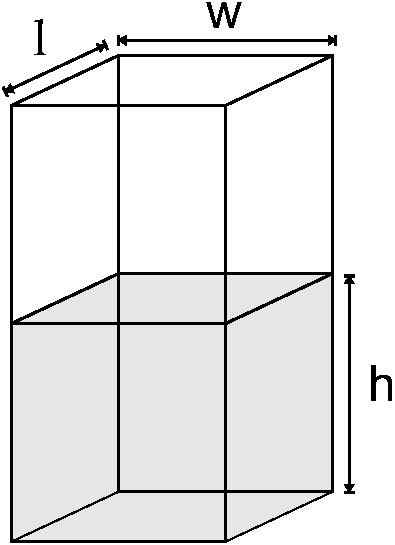
\includegraphics[width=6cm]{prism-lwh.pdf}
			\caption{Water Tank}
		\end{center}
	\end{figure}


	
\chapter{Solving Differential Equations}

	What we've been doing in the preceding chapters is, basically, solving differential equations. You're given an equation for the rate of change of something (height changes with time), and an initial value, and then have to see how the system evolves over time. 
	
	\section{Constant change}
	
	What if the rate of change is constant: our quantity changes at the same rate everywhere. For example: (see Eqn. \ref{square} and Table \ref{table:filling_data})
	
	\begin{equation}
		\frac{dy}{dx} = \frac{1}{2}
	\end{equation}

	\begin{equation}
		\label{test}
		y = \sqrt{5x}
	\end{equation}

	\begin{equation}
	\label{square}
	y = 5x^2
	\end{equation}

	\begin{table}[h!]
		\label{table:filling_data}
		\centering
		\begin{tabular}{||c | c | c||} 
			\hline
			time (s) & height measured (cm) & height modeled (cm)\\ [0.5ex] 
			\hline\hline
			1	& 0 & 6.57 \\
			7	& 10 & 16.00 \\
			12	& 20 & 23.86 \\
			16.8	& 30 & 31.72 \\
			21.5	& 40 & 39.58 \\
			26.2	& 50 & 45.87 \\ [1ex] 
			\hline
		\end{tabular}
		\caption{Combined time, measured data, and modeled data.}
	\end{table}

	\lstinputlisting[language=Python, frame=single, label={code:water-filling-noGraph}, caption={Model of a filling tube without graphing (\textit{water-filling-fd-noGraph.py})}]{water-filling-fd-noGraph.py}

 % Stop your text
 \end{document}
